\documentclass[10 pt]{article}

\usepackage[utf8x]{inputenc}
\usepackage{dsfont}
\usepackage{amsthm}
\usepackage{amsfonts}
\usepackage{tensor}
\usepackage{mathtools}
\usepackage[T1]{fontenc}
%\usepackage[spanish]{babel}
\usepackage[cm]{fullpage}
\usepackage{graphicx}
\usepackage{float}
\usepackage{bm}
\usepackage{setspace}
\usepackage{enumitem}
\usepackage{mdwlist}
\usepackage{parskip}
\usepackage{listings}
\usepackage{color}
%\usepackage{epstopdf}
\usepackage{tikz,datatool}
\usepackage{hyperref}

\newcommand{\HRule}{\rule{\linewidth}{0.5mm}}

\AtBeginDocument{
  \let\myThePage\thepage
  \renewcommand{\thepage}{\oldstylenums{\myThePage}}
}

\newcommand{\gra}{$^\text{o}$}
\newcommand{\dif}{\text{d}}
\newcommand{\avg}[1]{\left\langle #1 \right\rangle}
\newcommand{\ket}[1]{\left| #1 \right\rangle}
\newcommand{\bra}[1]{\left\langle #1 \right|}
\newcommand{\bket}[2]{\left\langle #1 \middle| #2 \right\rangle}
\newcommand{\der}[2]{\frac{\text{d} #1}{\text{d} #2}}
\newcommand{\prt}[2]{\frac{\partial #1}{\partial #2}}
\newcommand{\dert}[3]{\frac{\text{d}^#3 #1}{\text{d} #2^#3}}
\newcommand{\prtt}[3]{\frac{\partial^#3 #1}{\partial #2^#3}}
\newcommand{\dl}{\mathcal{L}}
\newcommand{\dha}{\mathcal{H}}
\newcommand{\vol}{\text{vol}}
\renewcommand{\vec}[1]{\pmb{#1}}

\newenvironment{algo}[1]
{  \begin{center}
   \mbox{
       \begin{minipage}{\textwidth}
           \begin{tabbing}
           \settabs
            #1
           \end{tabbing}
        \end{minipage}
    }
    \end{center}
}{}
\newcommand{\settabs}{mmm\=mmm\=mmm\=mmm\=mmm\=mmm\=\kill}

\DeclarePairedDelimiter\ceil{\lceil}{\rceil}
\DeclarePairedDelimiter\floor{\lfloor}{\rfloor}

\definecolor{mygray}{rgb}{0.4,0.4,0.4}
\definecolor{mygreen}{rgb}{0,0.5,0.25}
\definecolor{myorange}{rgb}{1.0,0.4,0}

\definecolor{clock0}{cmyk}{1,0,0,0}
\definecolor{clock1}{cmyk}{1,1,0,0}
\definecolor{clock2}{cmyk}{0,1,0,0}
\definecolor{clock3}{cmyk}{0,1,1,0}
\definecolor{clock4}{cmyk}{1,0,1,0}
\definecolor{clock5}{cmyk}{1,1,1,0}
\definecolor{clock6}{cmyk}{0,0,1,0}
\definecolor{clock7}{cmyk}{0,0,0,0.1}

\begin{document}

\lstset{
language=C++,
basicstyle=\ttfamily\color{black},
commentstyle=\color{mygray}\ttfamily,
frame=single,
numbers=left,
numbersep=5pt,
numberstyle=\tiny\color{mygray}\ttfamily,
keywordstyle=\color{mygreen}\ttfamily,
showspaces=false,
showstringspaces=false,
stringstyle=\color{myorange}\ttfamily,
tabsize=2,
emph={double,uint8_t,uint16_t,uint32_t,uint64_t,int8_t,int16_t,int32_t,int64_t},
emphstyle={\color{blue}\ttfamily}
}

\begin{center}
  \Large \textsc{Week 4: Monte Carlo simulation of hard spheres in the NPT ensemble}
\end{center}

\begin{center}
  \large \textsc{Francisco García Flórez}
\end{center}

\section{Pressure as a function of the packing fraction $\eta$}

\subsection{Solid initial configuration}

Firstly, we simulate a system of 108 particles starting from a FCC lattice of 3 by 3 by 3 unit cells, with a spacing of 1.5 units and spheres of radius 0.5.

\begin{figure}[H]
  \begin{center}
    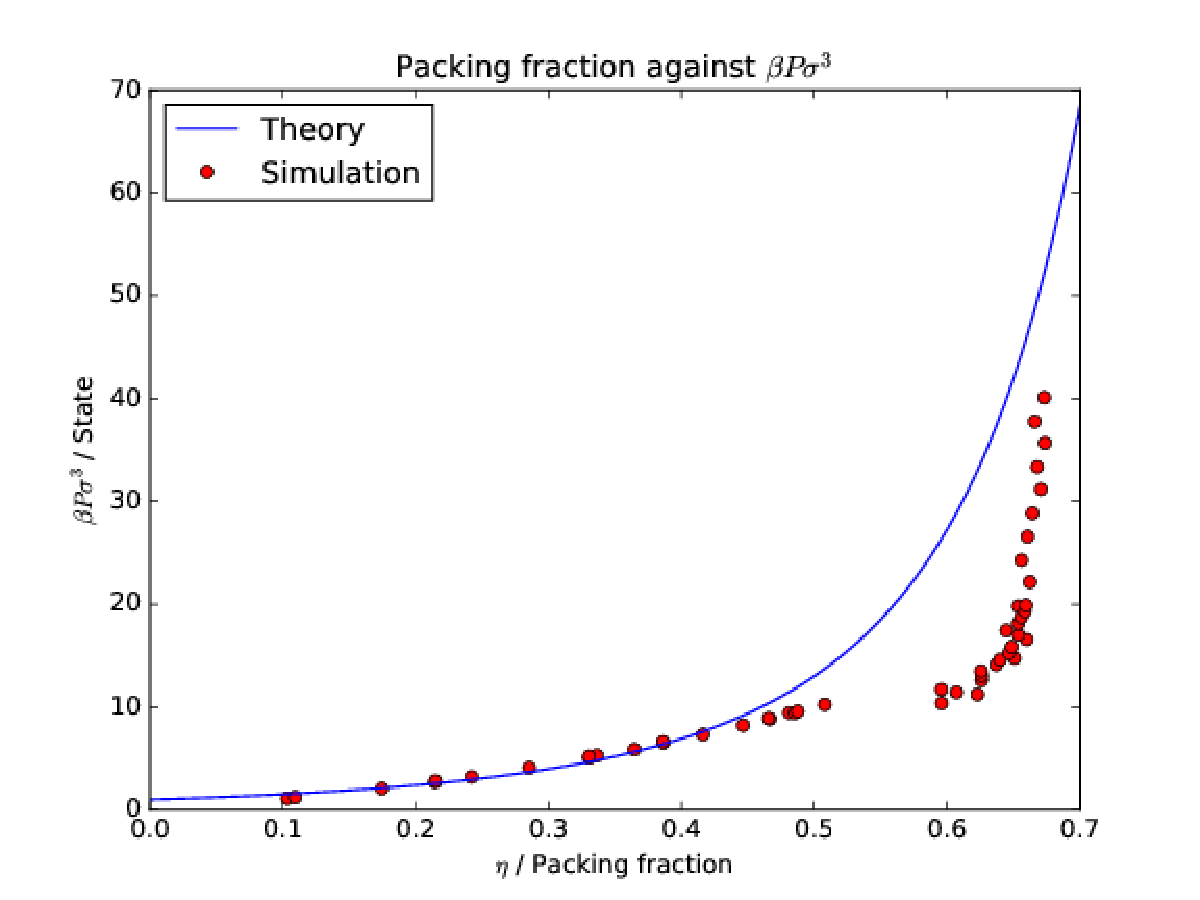
\includegraphics[width=0.7\textwidth]{../graphs/solid.pdf}
    \caption{Plot of the state as a function of the packing fraction.}
  \end{center}
\end{figure}

Where the blue line has been computed by the Carnahan and Starling equation of state:

$$ \frac{P_{cs}}{\rho k_B T} = \frac{1 + \eta + \eta^2 - \eta^3}{(1-\eta)^3} $$

This equation is only valid for the liquid phase, and as we could expect, for high enough pressures there's a phase transition from solid to liquid. In our simulation we find this transition to happen from $\eta \sim 0.56$ to $\eta \sim 0.59$, at the state $\beta P \sigma^3 \sim 10$.

After this discontinuity, the simulation points follow more or less CS equation of state, but shifted a certain amount. It is possible to improve this behavior by increasing the number of steps in the simulation, as it may have not reached equilibrium yet.

Of course, it cannot go higher than the maximum packing fraction of the FCC lattice (around 0.7), so it is expected to find some saturation effects close to this limit.

\subsection{Liquid initial configuration}

As before, we will simulate a system of the same characteristics, but starting now from a liquid phase of $\eta \sim 0.1$.

\begin{figure}[H]
  \begin{center}
    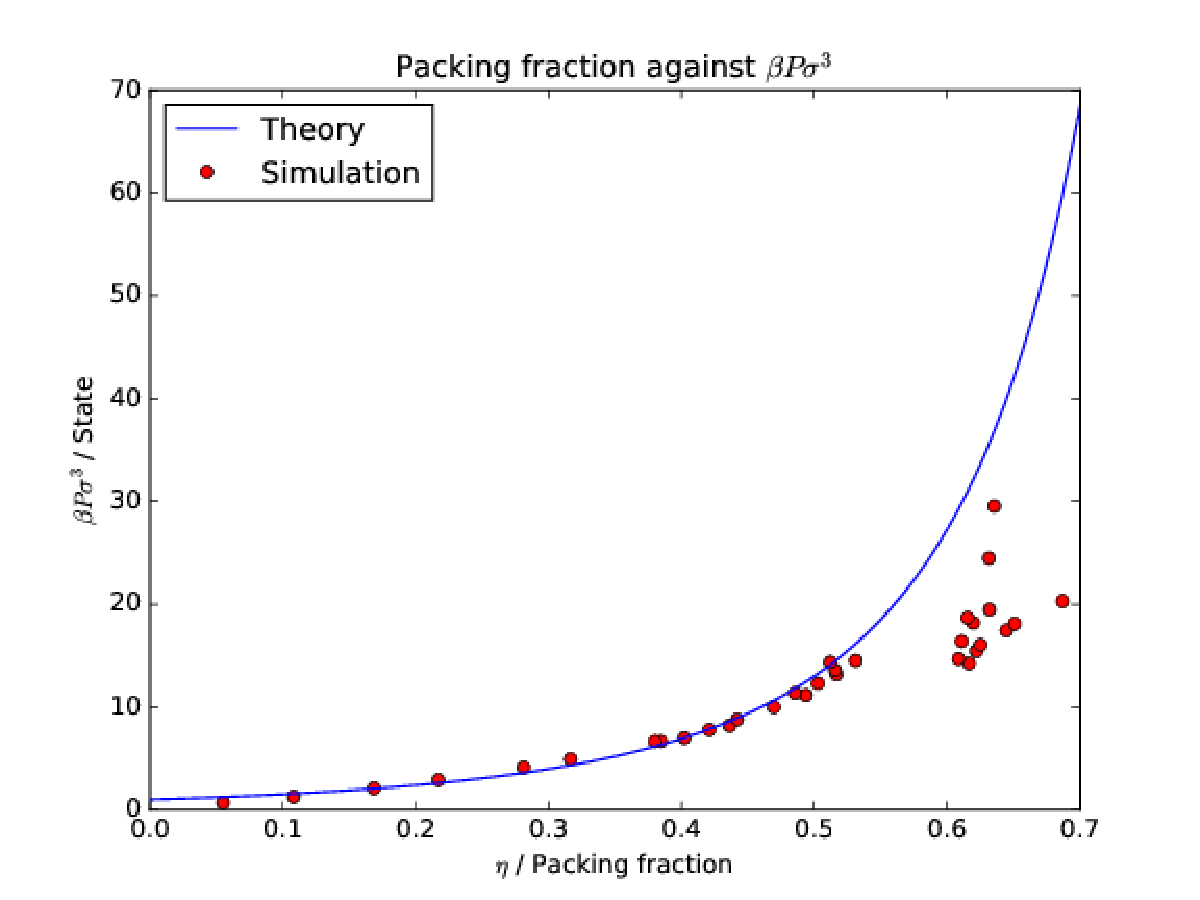
\includegraphics[width=0.7\textwidth]{../graphs/liquid.pdf}
    \caption{Plot of the state as a function of the packing fraction.}
  \end{center}
\end{figure}

In this case we find a much better agreement between theory and simulation for the liquid phase, probably related to the initial condition. We also find a slightly different value for the pressure, $\beta P \sigma^3 \sim 15$, what could be expected because of some hysteresis in the system. However, the gap in packing fraction during the transition has similar value than before.

Although, in this case it's more difficult to determine the behavior as a crystal, because the number of steps required to find equilibrium is too large.

\end{document}
